
\chapter{ \uppercase {Residual Monte Carlo Treatment of the Time Variable}}
\label{sec:time}
Another extension and improvement for the HOLO method described in Sec.~\ref{} is the time discretization
of the transport equation.  We have
incorporated the time variable into the ECMC method to improve efficiency over IMC, while still preserving the
accuracy of MC integration.  The main area of interest is in producing more accurate
resolution of radiation wave-fronts in optically
thin regions, where particles transport a long distance over a time step. In such regions, the MC
integration of the time variable by IMC can produce greater accuracy than an implicit
Euler discretization, which can produce artificially fast propagation of radiation in
space.   A potential application where this accuracy is important is stellar atmosphere calculations.  It is
noted that no adaptive refinement in time is performed, so maintaining exponential convergence
may not be possible.  However, we still expect the residual MC formulation of the ECMC method
to show improvement in efficiency over standard MC.

In the remainder of this chapter, the inclusion of the time variable into the ECMC trial
space is detailed, along with modifications to particle tracking and the ECMC algorithm.
The process of sampling, tracking, and tallies particle histories in time
is detailed in literature\cite{wollaber_review,fnc,wollaber_thesis,cj_thesis}, but
sufficient details are provided in this chapter.  
Finally, a new temporal closure for the LO equations is given, and results are compared to IMC for accuracy and
efficiency.  

\section{Modifications to the HO equations}
\label{sec:time_ho}

Inclusion of the time variable $t$ in the trial space used by ECMC allows for no discretization of the
transport operator $\B L$.  The transport operator, applied to the continuous intensity
$I$, becomes
\begin{equation}
    \B LI(x,\mu,t) = \frac{1}{c}\pderiv{I}{t}  + \mu \pderiv{I}{x} + \sigma_t I
\end{equation}
The emission source is still treated with an implicit Euler discretization, which is
similar to the approximation made in IMC.  The ECMC algorithm specified in
Sec.~\ref{sec:???} does not need to be modified.  However, the residual
source and trial-space representation are modified to include $t$.   Each batch is still estimating the error in the
current projection estimate $\tilde I(x,\mu,t)$, but the time variable must be included in the inversion of the $\B L$
operator.  
\subsection{The Doubly-Discontinuous Trial Space in Time}

It is necessary to define a new trial space that includes the time variable so that we can explicitly evaluate the residual.
The time variable has a similar representation to the LDD trial space used for the
spatial variable
in Sec.~\ref{sec:lo_closure_LDDTRIAL???}, but the solution is a constant value over
the interior of the time step. This step, doubly-discontinuous (SDD) trial space is defined as
\begin{equation}\label{eq:time_space}
    \tilde I(x,\mu,t) = \left \{ \begin{array}{cl}
        \tilde I^{n}(x,\mu)  & \quad t = t^n \\ 
        \overline I(x,\mu)  & \quad t \in (t^{n},t^{n+1}) \\               
      \tilde I^{n+1}(x,\mu)   &  \quad        t = t^{n+1}
    \end{array}           \right.
\end{equation}
where we have used $\overline I$ to denote the time-averaged LDFE \emph{projection} in $x$
and $\mu$ of the intensity over the interior of the time step;  the beginning and end of
time step projections are denoted $\tilde I^{n}$ and $\tilde I^{n+1}$, respectively.   An
illustration of $t$ for the SDD trial space, over the $n$-th time step, 
is depicted in Fig.~\ref{fig:dd_time}.    There is a projection error in using the LDFE projection to represent the intensity between time steps.  However, with
sufficient noise reduction and mesh resolution, this should be an acceptable error
compared to the large statistical noise of standard MC.
\begin{figure}[H]
    \centering
    \begin{center}
%        \resizebox{0.4\textwidth}{!}{
        \begin{tikzpicture}[scale=0.882, every node/.style={transform shape}]
            \draw (1.0,4.0) node[fill,circle,inner sep=0pt,minimum
            size=4.2pt] {};
            \draw [->] (1.6,4.25) -- (2.4,4.25) node[anchor=west] {$t$};
            \draw (1.0,0.4) -- (1.0,0.6) node[below, pos=0.4] {$t^{n}$};
            \draw (5.90,0.4) -- (5.90,0.6) node[below, pos=0.4] {$t^{n+1}$};
            \node at (3.6,3.06) {$\overline{I}_{HO}(x,\mu)$};
            \draw [thick] (1.0,0.5) -- (5.9,0.5) node[anchor=north west] {};
            \filldraw[color=black, fill=white] (1,2.450) circle (2.1pt);
            \draw (1.0,2.45) -- (5.90,2.45);
            \filldraw[color=black, fill=white] (5.9,2.450) circle (2.1pt);
            \draw (5.9,1.6) node[black,fill,circle,inner sep=0pt,minimum size=4.2pt] {};
            \node[anchor=west] at (5.9,1.6) {${\tilde{I}_{HO}^{n+1}}$};
        \end{tikzpicture}
 %   }
    \end{center}
    \caption{Step doubly-discontinuous representation of $t$ for the HO solution.}
    \label{fig:dd_time}
\end{figure}

The SDD trial space provides a projection for all the desired unknowns to exactly produce the moment
equations, i.e., the time-averaged, end of time step, and previous time step intensities;
temporally, these are the only unknowns that appear in equations that have
been integrated over a time step to produce a balance statement.  Another benefit of this
trial space is it allows for infrastructure for computing the residual from the
time-discrete case to be used directly.  This trial space has one major drawback:
only particle histories that reach $t^{n+1}$ contribute to the estimation of $\tilde
\epsilon^{n+1}$, and thus $I^{n+1}$.  This is undesirable in optically thick problems.
%where not much correction to the time-variable is necessary and accuracy is limited by the 
%the BE discretization of the This is troubling, because in such problems you don't need much correction in
%the time variable.

REWRITE: Possibly move this to the future work section
Alternatively, an LDFE representation could be used in the time
variable. The linear representation should produce less noise because all particle tracks
contribute to the slope, rather than just those that reach the end of the time step,
although it would produce an approximate projection error for the end of time step
intensity that is not produced with a discontinuity at the end of the time step.  The
linear representation in time would also produce a more accurate reconstruction of the
scattering source in time.  However, a linear representation requires the sampling
algorithm to be significantly modified because the L$_1$ integral for computing the
residual magnitude is now significantly complicated by the tri-linear function.  A
possible way to sample this source is discussed in Appendix??? for completeness, but it has
not been rigorously investigated.

\subsection{Residual Source Definition and Sampling}
\label{sec:time_sampling}

The residual is defined as $r = q - \B L \tilde I(x,\mu,t)$, where
\begin{equation}
    q=\left(\sigma_a a c (T_{LO}^{n+1})^4(x) + \sigma_s\overline\phi_{LO}\right)
\end{equation}
is a constant in time and provided by the LO solver. We have assumed a constant reconstruction for the scattering source
in time.
Evaluation of the residual with Eq.~\eqref{eq:time_space} for $I$ produces a uniform source in time, as well as a $\delta$-function source at the
beginning and end of the time step.  We write the residual source in terms of three components:
\begin{equation}
    r(x,\mu,t) = \overline r(x,\mu)  + r^{n}(x,\mu)\delta^+(t-t^{n}) +
    r^{n+1}(x,\mu)\delta^-(t - t^{n+1}),
    \quad t\in[t^{n},t^{n+1}]
\end{equation}

We will look at each component individually.  
The first residual term is a constant in time with representation
\begin{equation}
    \overline r(x,\mu) = q  - \mu \pderiv{\overline I(x,\mu)}{x} - \sigma_t \overline
    I(x,\mu)
\end{equation}
Evaluation of the above function produces both face and interior volumetric components (as
in the time discrete case), respectively labeled $\overline r_{\text{face}}$ and
$\overline{r}_{\text{int}}$.  To sample $x$ and $\mu$ from the face and volume distributions, the
same rejection procedure can be used as for Eq.~\eqref{eq:???} and detailed
in~\cite{jake}.    The time variable can then be sampled uniformly over the time step,
i.e., $t=t^n + \eta \Delta t$, where $\eta$ is a uniform random variable with support
$(0,1)$.

The second source has definition
\begin{equation}
    r^{n}(x,\mu) = -\frac{1}{c}\pderiv{\overline{I}(x,\mu)}{t}\bigg|_{t=t^{n}}
    =-\frac{1}{c}\left(\overline I(x,\mu) - \tilde I^{n}(x,\mu)\right)
\end{equation}
This source is a LDFE space and angle volumetric source.
The rejection sampling procedure is used to sample $x$ and $\mu$.
All particles sampled from this source begin tracking with $t=t^{n}$.

The final source term is
\begin{equation}
    r^{n+1}(x,\mu) = -\frac{1}{c}\pderiv{\overline{I}(x,\mu)}{t}\bigg|_{t=t^{n+1}}
    =-\frac{1}{c}\left(\tilde I^{n+1}(x,\mu) - \overline I(x,\mu)\right).
\end{equation}
The source $r^{n+1}$ can be treated using the
same analytic treatment as the outflow face source in the LDD
trial space, as discussed in Sec.~\ref{sec:ldd_mc} and derived in
App.~\ref{sec:face_err_deriv}.  The source at the end of the time step is
never sampled, because its contribution to $I^{n+1}$ can be analytically computed.  To treat the sources this way, the solution for $\tilde I^{n+1}(x,\mu)$ is
initialized to the value of $\overline I(x,\mu)$ before a batch of particles begins.
Then, error particles that reach the end of the time step, referred to as ``census''
particles, contribute a standard score to the projection $\tilde I^{n+1}(x,\mu)$.

With these definitions, it is thus only necessary to sample from two sources.  We apply
the systematic-sampling algorithm described in Sec.~\ref{sec:systematic_sampling}.  The
number of histories sampled from each space-angle element is proportional to the magnitude
of the residual within that cell, and a minimum number of histories is sampled from cells
with a non-zero residual.  Then, composite-rejection sampling is used to sampled from the
appropriate source.  The algorithm for each sample, from $x-\mu$ element $i$, is 
\begin{enumerate}
    \item Sample two random numbers $\eta_1$, $\eta_2\sim U(0,1)$ 
    \item If $\eta_1 < \|r_i^{n}\|_1/(\|r_i^{n}\|_1 + \|\overline{r_i}\|_1)$:
    \begin{itemize}
        \item Sample $(x,\mu)$ from $r_i^{n}$ volumetric source using rejection sampling
        \item Set $t=t^n$
    \end{itemize}
\item Else, sample from $\overline r$ source:
    \begin{enumerate}
        \item \label{itm:time_step}Sample $t$ uniformly over $(t^{n},t^{n+1})$.
        \item If $\eta_2 < \|\overline{r}_{i,\text{face}}\|_1/\|\overline{r}_{i}\|_1$:
            \begin{itemize}
                \item Sample $(x,\mu)$ from $\overline r_{i,\text{face}}$ face source using rejection
            \end{itemize}
        \item Else:
            \begin{itemize}
                \item Sample $(x,\mu)$ from $\overline r_{i,\text{int}}$ volumetric source using rejection
            \end{itemize}
    \end{enumerate}
\end{enumerate}
where all L$_1$ norms are over element $i$.  All L$_1$ integrals can be analytically
evaluated using the same numerics as in the
time-discrete case because each residual component is either a volumetric or face
component.  

\subsection{Importance Sampling on Interior of Time Step}
\label{sec:imp_sampling}

As an attempt to reduce variance in the estimate of $\tilde \epsilon^{n+1}(x,\mu)$, we use
important sampling in the time variable.  Systematic sampling is still used for
determining the cell of interest, and sampling as described above is used to determine
which source is sampled, based on the appropriate probabilities described in the previous
section.  However, when the interior source $\overline r(x,\mu)$ is sampled, we use
importance sampling for the conditional sampling of the uniform time step.  The goal is to ensure that some
histories reach the end of the time step.  In order to do this, we sample from a modified
PDF such that a fraction $p_{surv}$ of particles sampled from $\overline r(x,\mu)$ are born
with $t\in(t^{surv},t^{n+1})$.  We define $t^{surv}=t^{n+1}-M/(c\sigma_t)$, where $M$ is the desired
number of MFP of travel the particle will undergo from the end of
the time step (e.g., 2 or 3).  The weights of particles sampled from this
distribution must be modified to prevent biasing of the solution.  This only affects
Step~\ref{itm:time_step}.

The new PDF to be sampled from is
\begin{equation}
    f^*(t) = \left\{ \begin{array}{cl}
        \frac{\ds 1 - p_{surv}}{\ds t^{surv} - t^n} &\quad 0 < t < t^{surv} \\ 
        \frac{\ds p_{surv}}{\ds t^{n+1} - t^{surv}} & \quad t^{surv} \leq t < t^{n+1}  \\
        0 & \quad \text{elsewhere}\end{array}  \right.
\end{equation}
The original PDF is $f(t)= 1/\Delta t$, for $t\in(t^{n},t^{n+1})$.  Thus, using the
standard procedure for importance sampling\cite{shultis_mc}, the starting time $t_{\text{start}}$ is sampled from
$f^*(t)$, and then weights are multiplied by the factor
$f(t_{\text{start}})/f^*(t_{\text{start}})$.  This procedure is not perfect in that if a
particle is moving from an optically thin to an optically thick
region, it is not guaranteed to reach census. However, this case does not introduce bias.

\subsection{Tracking and Tallying in Time}

Because our LO equations will be integrated over the time step, we only need to
perform MC tracking for $t\in[t^{n},t^{n+1}]$.  
The initial time for the particle is
sampled as described in the previous section. In inverting the $\B L$ operator, particles
are tracked until they reach the end of the time step.  Path lengths are sampled or the
weight is exponentially attenuated as before (e.g., Sec.~\ref{sec:???}).  As a particle
travels from position $x_{o}$ to $x_{f}$, with direction $\mu$, the time is updated as 
\begin{equation}
    t^{f} = t^{0} + \frac{|x_{f} - x_{o}|}{c \mu}
\end{equation}
where $c$ is the speed of light. For analog path-length sampling, if $t^{f}>t^{n+1}$ then $t^{f}$ is adjusted to $t^{n+1}$
and the path length is adjusted accordingly.  For continuous weight deposition, particles
are only tracked until they reach $t^{n+1}$.  A proof that this process of tracking
particles is a MC solution to an integral equation that is exactly inverse to the $\B L$ operator is
detailed in~\cite{cj_thesis,shultis_paper_cj_cites???}.  

Tallies must be adjusted to account for the averaging over the time step, and to compute the
intensity at the end of time step.  To produced the time-averaged representation
$\overline I(x,\mu)$, requires estimators for the average, $x$, and $\mu$ moments of the
error, e.g.,
\begin{equation}
    \overline\epsilon_{x,ij} = \frac{1}{\Delta t} \frac{6}{h_j}
    \int\limits_{t^{n}}^{t^{n+1}} \!\!\dd t \!\!\!
    \int\limits_{\xl}^{\xr} \!\!\!\!\! \dd x
    \hspace{-0.081in}\int\limits_{\mu_{j-1/2}}^{\mu_{j+1/2}} \hspace{-0.107in} \dd \mu
    \;\left(\frac{x - x_j}{h_{i}}\right) \epsilon(x,\mu,t)
\end{equation}
with a similar definition for the average and $\mu$ moments.  The estimators are defined
as
\begin{equation}
    \hat{\overline \epsilon}_{x,ij} =\frac{1}{N_{hist}} \frac{6}{\Delta t h_i} \sum_{n=1}^{N_{hist}}
    \frac{s_n}{h_{i}h_{j}} w_j \left(x_c - x_i\right),
\end{equation}
where the magnitude of the weights produce the L$_1$ integral over all phase space, i.e.,
\begin{equation}
\sum\limits_{n=1}^{N} w_n = \| r(x,\mu,t) \|_1 \equiv 
    \int\limits_{t^{n}}^{t^{n+1}} \!\!\dd t \!\!\!
    \int\limits_{\xl}^{\xr} \!\!\!\!\! \dd x
    \hspace{-0.081in}\int\limits_{\mu_{j-1/2}}^{\mu_{j+1/2}} \!\!\!\!\dd \mu\;
    |r(x,\mu,t)|.
\end{equation}
Here, $x_c$ is the center of the $n$-th
path length, and $s_{n}$ is the path length for the $n$-th path length in the $x-\mu$ cell.

Moments of $I^{n+1}(x,\mu)$ must be estimated to represent the end of time step intensity.
For example, the $x$ moment for the $ij$-th cell of the error at the end of time step is
\begin{equation}
    \epsilon^{n+1}_{x,ij} = \frac{6}{h_i} \iint\limits_{\mathcal{D}_{ij}} \left(\frac{x
    - x_i}{h_i}\right) \epsilon(x,\mu,t^{n+1}) \dd x \dd \mu
\end{equation}
The estimators for these moments are a generalization of the census
tallies used in IMC~\cite{wollaber_review,wollaber_thesis}.  The tallies are based on the
definition of the intensity as $I(x,\mu,t) = c h \nu N(x,\mu,t)$ given in
Eq.~\eqref{???}, similar to collision estimators~\cite{shultis_mc,mcnp}.  The census estimator for the $x$ moment is
\begin{equation}
    \hat\epsilon^{n+1}_{x,ij} = \frac{1}{N_{hist}} \frac{6}{h_j h_i} \sum_{n=1}^{N_{hist}}
    c w_j  \left(x_{c} - x_{i}\right)
\end{equation}
Similar tallies are defined for the other space-angle moments. These tallies can be
exceptionally noisy because only particles that reach the end of the time step contribute.


\section{Closing the LO Equations in Time}

The LO equations must be closed in time consistently with the HO
equations.   Previous work has enforced
consistency in time by adding a local artificial source to the time-discretized LO
equations in each cell~\cite{holo_rh}.  This
source was approximated based on the difference between the exact HO integral of the time
derivative and the approximate representation in the LO equations. The advantage
of this form is that the LO solver exclusively deals in
time-averaged unknowns for the radiation terms in the equations.  However, if the problem
is strongly non-linear or the time-averaged and time-edge
values differ greatly, this may become unstable.

We will alternatively use a
parametric closure in the time variable, similar to the spatial closures discussed in the
Sec.~\ref{???}.  The time-integrated LO equations can be written exclusively in terms
of time-averaged unknowns.  This closure
produces LO equations that have the same numerical difficulty to solve as the BE,
fully-discrete LO equations, but
have the potential to preserve the accuracy of the MC integration in time, upon non-linear
convergence of the system.   A closure relation is used to eliminate
the end of time step moments present from the time derivative term.   We will investigate different parametric forms of the closure for robustness.   Once the time-averaged unknowns have been calculated,
the time closures can be used to convert the time-averaged unknowns to end-of-time-step
values.

REWRITE THIS SENTENCE
One potential benefit of the time closure parameters is that $\overline I^{HO}$ will be
most different from $I^{HO,n+1}$ in problems that are optically thin.  In such problems,
$\sigma_a$ is small, leading to an optically thin problem.  However, there may be
difficulties in the MPV problems where the problems are tightly coupled and nonlinear, but
can lead to a large change over a time step.

REWRITE: I think most of these paragraphs can be moved to intro

\subsection{Derivation of Time-Averaged Moment Equations}

The time-continuous radiation equations are integrated in space and angle the same as
before.  For example, the $L$ and $+$ moment equation is
\begin{multline}
    \frac{1}{c}   \pderiv{ }{t} \mom{\phi}^+_L - 2\left({\mu}_{i-1/2} I_{i-1/2}\right)^+ + \mom{\mu I}^+_{L,i} 
    + \mom{\mu I}^+_{R,i} +  \sigma_{t,i} h_i \mom{\phi}_{L,i}^{+} -  \frac{\sigma_{s,i} h_i}{2} \left( \mom{\phi}_{L,i}^{+} +
  \mom\phi_{L,i}^{-}\right) \\ = \frac{h_i}{2} \mom{\sigma_a a c T^4}_{L,i} 
\end{multline}
This equation is then integrated over the time step, and the emission source is assumed
implicit.  The same manipulations can be
performed on the streaming term to form angular consistency terms, but the weighting fluxes are now
time-averaged values.  Thus, the angular consistency terms are computed with $\overline I(x,\mu)$.  
The equations with time-averaged consistency terms are
\begin{multline}\label{eq:t_moml_ex}
    \frac{\mom{\phi}_{L,i}^{+,n+1} - \mom{\phi}_{L,i}^{+,n}}{c \Delta t}
    -2\overline {\mu}_{i-1/2}^{\,+} \overline \phi_{i-1/2}^{\,+} + \overline{\cur {\mu}}_{L,i}^{+}
  \mom{\phibar}_{L,i}^{+}
  +  \overline{\cur\mu}_{R,i}^{+}
  \mom{\phibar}_{R,i}^{+} +  \sigma_{t,i}^{n+1} h_i 
  \mom{\overline\phi}_{L,i}^{n+1,+} \\-  \frac{\sigma_{s,i} h_i}{2} \left( \mom{\phibar}_{L,i}^{+} +
  \mom{\phibar}_{L,i}^{-}\right) = \frac{h_i}{2} \mom{\sigma_a^{n+1} a c T^{n+1,4}}_{L,i},
\end{multline}
These equations are exact at this point.  The BE approximation is used for the temperature
terms in the material energy equations, but the radiation energy deposition is a
time-averaged valued.
REWRITE: Maybe add material energy equation

\subsection{Parametric Time Closure}
%\subsection{Alternative time discretization}
%\label{sec:time}
%
The closure relations in time are different than the closure relations for the spatial
variable because we do not have a slope in time.  The following closure is a modified diamond
relation:
\begin{equation}\label{eq:tc_diam}
    I^{n+1} = 2\gamma \overline{I} - I^{n}
\end{equation}
where $\gamma$ is the closure factor and $\overline{I}$ is the time-averaged
intensity.  A modified BE discretization can also be used:
\begin{equation}\label{eq:tc_avg}
    I^{n+1} = \gamma \overline{I}
\end{equation}

The chosen closure relation must be used to eliminate the unknowns at $t^{n+1}$ from each
of the LO moment equations, with the values from the previous time step taken as a known quantity.  Thus, it is necessary to have a closure relation for each moment and half
range, producing four closure parameters per spatial cell.  The closure relations for the
$L$ moment and the modified diamond relation are
\begin{equation}\label{eq:tc_diam_l}
    \mom{\phi}_{L,i}^{\pm,n+1} = 2 \gamma_{L,i}^{\pm}\mom{\overline\phi}_{L,i}^{\pm} -
    \mom{\phi}_{L,i}^{\pm,n}
\end{equation}
with equivalent definitions for the $R$ moment.  Substitution of the above equation into
Eq.~\eqref{eq:t_moml_ex}
\begin{multline}
    \frac{2}{c\Delta t}\left[ \gamma_{L,i}^{+} \mom{\phi}_L^{+,n+1} - \mom{\phi}_L^{+,n} \right]
    -2\overline {\mu}_{i-1/2}^{\,+} \overline \phi_{i-1/2}^{\,+} + \overline{\cur {\mu}}_{L,i}^{+}
  \mom{\phibar}_{L,i}^{+}
  +  \overline{\cur\mu}_{R,i}^{+}
  \mom{\phibar}_{R,i}^{+} +  \sigma_{t,i}^{n+1} h_i 
  \mom{\overline\phi}_{L,i}^{+} \\-  \frac{\sigma_{s,i} h_i}{2} \left( \mom{\phibar}_{L,i}^{+} +
  \mom{\phibar}_{L,i}^{-}\right) = \frac{h_i}{2} \mom{\sigma_a^{n+1} a c T^{n+1,4}}_{L,i},
\end{multline}
The other moment equations are analogously defined.  

The value of $\gamma_{L,i}^+$, $\gamma_{R,i}^+$, $\gamma_{L,i}^-$, and $\gamma_{R,i}^-$
can be computed by substituting the trial-space representation of $I^{HO}(x,\mu,t)$ into
Eq.~\eqref{eq:tc_diam_l} and its analogs.


\section{Computational Results}

We will test the HO time closure for several problems that characterize potential physics
regime.  Throughout this
section, for the HOLO method, results that use the backward Euler discretization are indicated with HOLO-BE and the MC-based time
closure are indicated with HOLO-TC, where applicable.  For simplicity, all HOLO results
have used the lumped-relation in the LO radiation moment equations to preserve positivity. We will compare sample statistics
and accuracy against IMC simulations.
The systematic sampling algorithms detailed in Sec.~\ref{sec:systematic_sampling} and
Sec.~\ref{sec:time_sampling} were used for all HOLO results in this
section.  In
the algorithm the average is set to the floor value and slopes to zero in such cells.

\subsection{Near-Void Problem}

For the first problem, the material properties
are uniform throughout a 2.0 cm wide domain with $\rho c_v = 0.01374$ Jks cm$^{-3}$ keV$^{-1}$, $\sigma_a=10^{-6}$ cm$^{-1}$, and $\sigma_s=0$ \invcm.
The material and radiation are initially in equilibrium at a temperature of $0.01$ keV.
An isotropic incident intensity with $T_r = 0.150$ keV is applied
at $x=0$ for $t>0$; the incident intensity on the right boundary is $0.01$ keV.  The simulation end
time is 0.003 sh.  Because the problem is optically thin, no importance sampling on the
interior of the time step is used.   For this problem, we expect IMC to be accurate
because the small opacity leads to the material energy equation being mostly uncoupled.  
\begin{figure}[H]
  \centering
    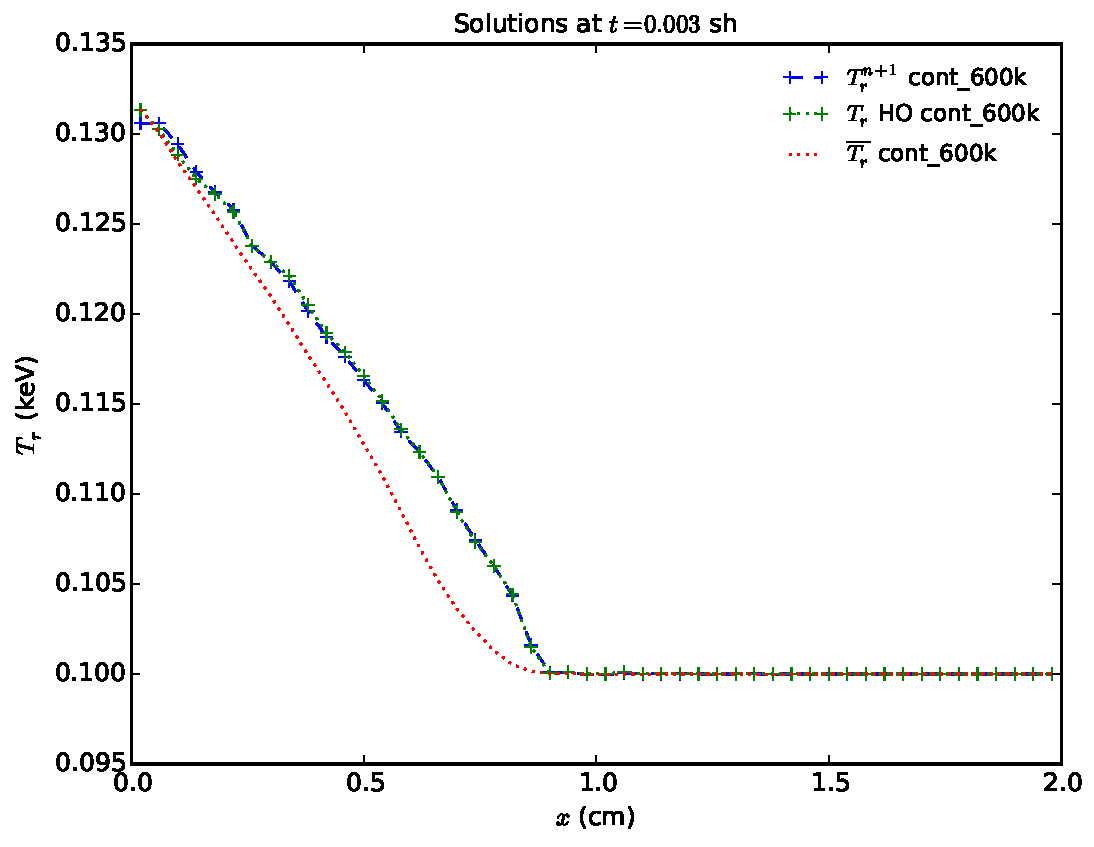
\includegraphics[width=0.65\textwidth]{void_imc_compare.pdf}
    \caption{\label{fig:void_imc_compare} Comparison of radiation energy densities of IMC
    and HOLO method for the HO time closure and a BE discretization.}
\end{figure}

A comparison of the cell-averaged radiation energy densities $E_r$ for IMC and the HOLO
method with the diamond-like HO time closure are depicted in Fig.~\ref{fig:void_imc_compare},
both for the time-averaged solutions and end-of time step values, from the final time
step.  The end of time step value for the HOLO method with a BE discretization is also depicted.
For the HOLO results, three ECMC batches were performed with
a total of $3\times10^6$ histories per time step and the IMC results were generated with
$12\times10^6$ histories per time step. 
The minimum number of histories for any sampled space-angle cell, $N_{cut}???$ in
 Eq.~\eqref{???}, is 20 for all HOLO simulations.
The spatial meshs had 100 spatial cells and both
HOLO results used 20 $\mu$ cells.  
The MC treatment of the time
variable and the closure of the LO equations allow the LO results to correctly reconstruct
the wave-front location of IMC, whereas the BE discretization artificially propagates
energy.   Although not plotted, the results were visually equivalent for either the diamond-like or implicit-like
closures in this problem.  This is because the problem is nearly linear due to the small
opacities, so the HO moments are reproduced accurately, independent of the chosen closure
equation.

A comparison of similar results, but plotted as radiation temperatures, is plotted in
Fig.~\ref{void_temp_compare}.  By plotting
proportional to the fourth-root of the radiation energy density, the noise at low
magnitudes past the wave-front are more apparent in the 3 batches and $\Delta t = 0.001$
case.  This
noise is small relative to the scale of $E_r$, but it demonstrates a defficiency of
the trial space.  The cause is from the step representation over the time step leading to
particles sampled near the wave-front with a time near $t^{n}$ that travel into the
equilibrium region.  It is noted this is not a bias, but rather an undersampling; if
sufficient histories were performed there would be negative particles that canceled out this
error.  This effect is significantly reduced when a smaller time step is taken, although
it increases the projection error between time steps. 

For the case of a single batch, 
there is less noise past the wavefront because the
choice of $I^{n}(x,\mu)$ and an initial guess for $I^{n+1}(x,\mu)$ prevents most particles from
traveling past what the physical transport should allow.  The discrepancy betweeen the IMC
and HOLO solution near the foot of
the wave is a result of the spatial discrepancy between the LDFE HO projection and the
lumped LD LO equations; this dispersion is not present in the HO solution.  This
discrepancy can also lead to some negativities in the LD representation of
$\phi^{n+1}(x)$, which are set to the floor value for the next calculation. 


\begin{figure}[H]
  \centering
    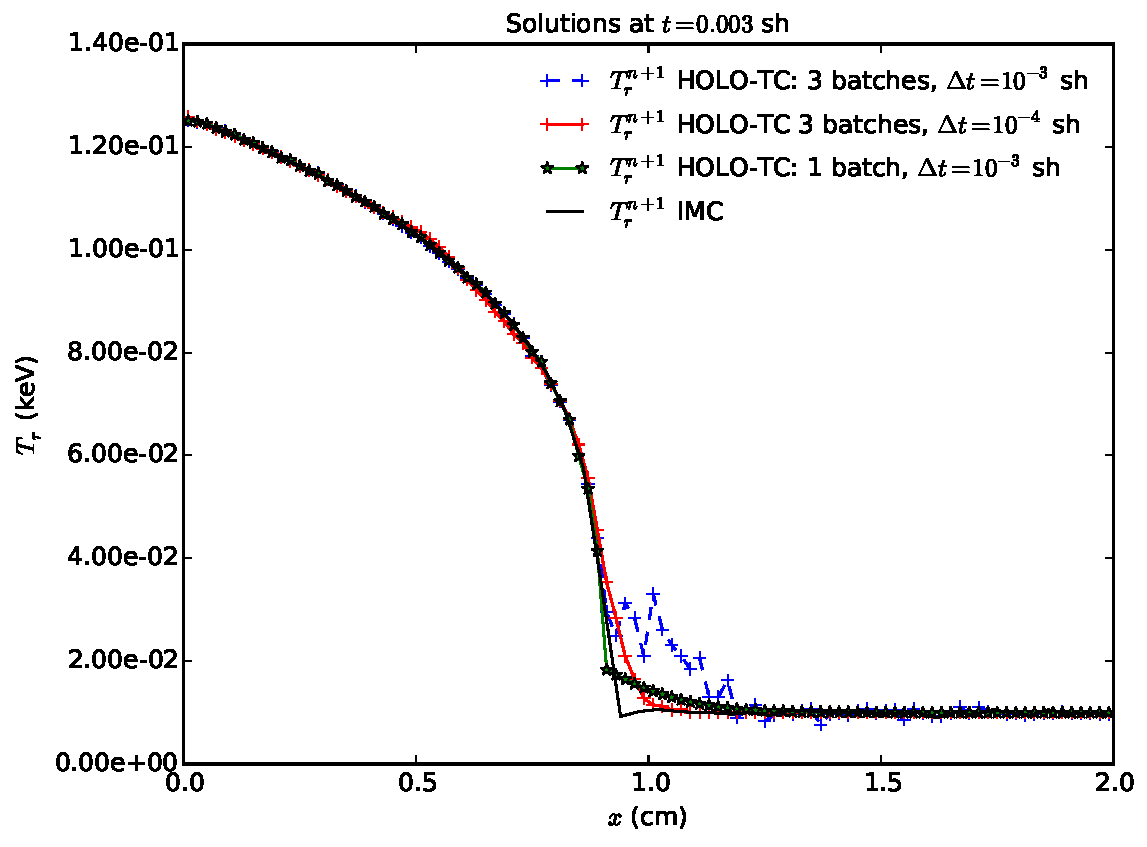
\includegraphics[width=0.75\textwidth]{void_temp_batch_compare.pdf}
    \caption{\label{fig:void_temp_compare} Comparison of radiation temperatures of IMC and
    the HOLO method for different time step sizes and numbers of batches, for the
near-void problem.}
\end{figure}

\begin{figure}[H]
  \centering
    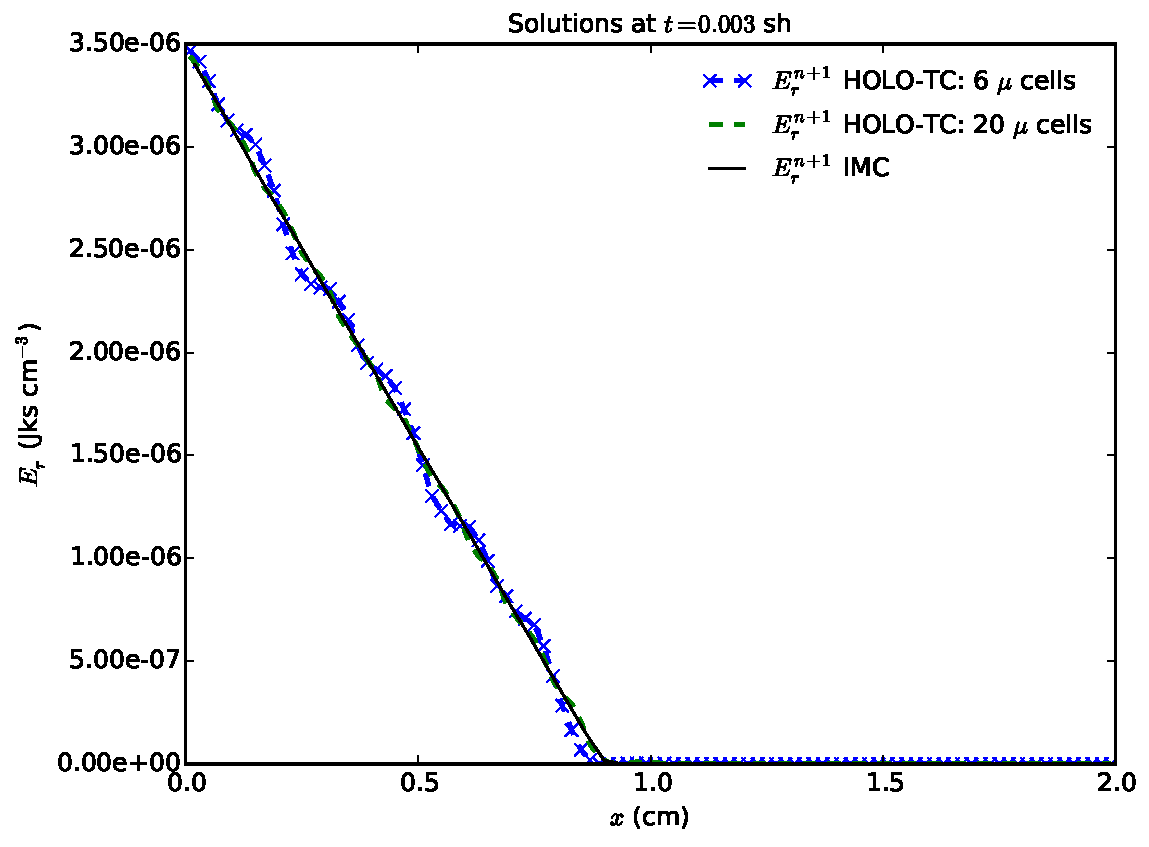
\includegraphics[width=0.75\textwidth]{void_ang_compare.pdf}
    \caption{\label{fig:bumps} Comparison of radiation energy densities for
    the HOLO method with different numbers of $\mu$ cells. $\Delta t=0.001$ sh, for
near-void problem.}
\end{figure}

Figure.~\ref{fig:bumps} compares radiation energy densities for various numbers of $\mu$
cells.  At coarser mesh sizes, the imprinting of the mesh is visible in the location of
the wave-front.  This is a result of the projection onto the space-angle mesh between time
steps.  As the mesh is refined, the solution converges towards the IMC solution.  
Smaller time step sizes can increase the mesh imprinting because the projection onto the
trial space happens more often.  However, it is important
to note that the mesh imprinting will be reduced as $\sigma_a$ is increased and
absorption-emission events smooth the angular intensity across each time step.

We have computed FOM statistics using Eq.~\eqref{eq:fom} with 20 independent runs for each
problem set up and parameters.  The statistics are computed based on the time-averaged
radiation energy densities.  
It is noted that the FOM results for each time step size are normalized to the IMC results within
that table.  
The results are compared for two different time step sizes 
in Tables~\ref{tab:void_long} and \ref{tab:void_short}.   The different number of batches for the HOLO methods are
indicated in parenthesis next to the method names.  The results demonstrate that IMC can
be more efficient than the ECMC method at longer time step sizes.  This is a limiting case; because minimal absorptions are
occuring in this problem, the IMC method is just advancing the initially sampled census particles
between time steps, so there is negligible resampling of the phase space.  Whereas, ECMC
must resample the residual source and the step trial-space on the interior of the tiem
step has a larger truncation error. At smaller time step sizes,
the ECMC method, particularly for the single batch case, becomes more efficient than IMC.
% THESE RESULTS ARE FOR THE CENSUS CASE
%\begin{table}[H]
%\centering
%\caption{\label{tab:void_long} \textbf{Comparison of sample statistics for the Near-Void
%    problem and $\Delta t = 0.001$ sh.   Simulation end time is $\mathbf{t=0.003}$ sh.}}
%\vspace{-0.1in}
%\begin{tabular}{|c|ccc|ccc|}\cline{2-7}
%    \multicolumn{1}{c|}{}       & \multicolumn{3}{|c|}{\ss} &
%    \multicolumn{3}{|c|}{\FOM} \\ \hline
%hists./step   & IMC & HOLO-TC (1) & HOLO-TC (3) &  IMC   & HOLO-TC(1) & HOLO-TC(3) \\ \hline
%   300,000    & 1.01\% & 1.39\% & 1.39\%    &       1.00  & 0.53       & 0.53       \\
%  3,000,000   & 0.32\% & 0.25\% & 0.46\%     &      0.97  & 1.68       & 0.48      \\ \hline
%\end{tabular}
%\end{table}
%
%\begin{table}[H]
%\centering
%\caption{\label{tab:void_short} \textbf{Comparison of sample statistics for the Near-Void
%    problem and $\Delta t = 10^{-4}$ sh.   Simulation end time is $\mathbf{t=0.003}$ sh.}}
%\vspace{-0.1in}
%\begin{tabular}{|c|ccc|ccc|}\cline{2-7}
%    \multicolumn{1}{c|}{}       & \multicolumn{3}{|c|}{\ss} &
%    \multicolumn{3}{|c|}{\FOM} \\ \hline
%hists./step   & IMC & HOLO-TC (1) & HOLO-TC (3) &  IMC   & HOLO-TC(1) & HOLO-TC(3) \\ \hline
%   30,000     & 3.15\%  & 0.54\% & 1.99\%       &  1.00  & 34.40      & 2.51        \\
%  300,000     & 1.01\%  & 0.13\% & 0.40\%       &  0.97  & 53.48      & 6.09        \\ \hline
%\end{tabular}
%\end{table}


\begin{table}[H]
\centering
\caption{\label{tab:void_long} \textbf{Comparison of sample statistics for the
    time-averaged radiation energy densities, of the last time step, for the near-void
    problem and $\Delta t = 0.001$ sh.   Simulation end time is $\mathbf{t=0.003}$ sh.}}
\vspace{-0.1in}
\begin{tabular}{|c|ccc|ccc|}\cline{2-7}
    \multicolumn{1}{c|}{}       & \multicolumn{3}{|c|}{\ss} &
    \multicolumn{3}{|c|}{\FOM} \\ \hline
hists./step   & IMC & HOLO-TC (1) & HOLO-TC (3) &  IMC   & HOLO-TC(1) & HOLO-TC(3) \\ \hline
   300,000    & 0.27\% & 0.27\% & 0.45\%     & 1.00       &  0.96     & 0.35      \\
  3,000,000   & 0.09\% & 0.06\% & 0.15\%     & 1.04       &  2.19     & 0.33      \\ \hline
\end{tabular}
\end{table}

\begin{table}[H]
\centering
\caption{\label{tab:void_short} \textbf{Comparison of sample statistics for the
    time-averaged radiation energy densities, of the last time step, for the near-void
    problem and $\Delta t = 10^{-4}$ sh.   Simulation end time is $\mathbf{t=0.003}$ sh.}}
\vspace{-0.1in}
\begin{tabular}{|c|ccc|ccc|}\cline{2-7}
    \multicolumn{1}{c|}{}       & \multicolumn{3}{|c|}{\ss} &
    \multicolumn{3}{|c|}{\FOM} \\ \hline
hists./step   & IMC & HOLO-TC (1) & HOLO-TC (3) &  IMC   & HOLO-TC(1) & HOLO-TC(3) \\ \hline
   30,000     & 2.46\%  & 0.44\% & 1.65\%       &  1.00  & 31.07      & 2.22       \\
  300,000     & 0.80\%  & 0.12\% & 0.37\%       &  0.95  & 43.66      & 4.47       \\ \hline
\end{tabular}
\end{table}



\section{Optically Thin Problem}

We modify the problem in the previous problem by increasing the absorption cross section to 0.2
\invcm; all other problem parameters are the same.  Radiation temperatures at the end of
the last time step are compared for IMC, HOLO-TC, and HOLO-BE in
Fig.~\ref{fig:thin_temp_compare}.  The HOLO-TC and HOLO-BE results were generated with 30
$\mu$ cells, and all spatial meshes used 200 cells.  At smaller time step sizes, the
effects of mesh imprinting are slightly apparent in the HOLO-TC results, leading to more
dispersion near the wave-front.  For $\Delta t=0.005$ sh, there is good agreement between
the HOLO-TC results and IMC.  As in the previous problem, the HOLO-BE results do not accurately capture
the wavefront location. IMC demonstrates substantial statistical noise in the equilibrium region.

\begin{figure}[H]
  \centering
    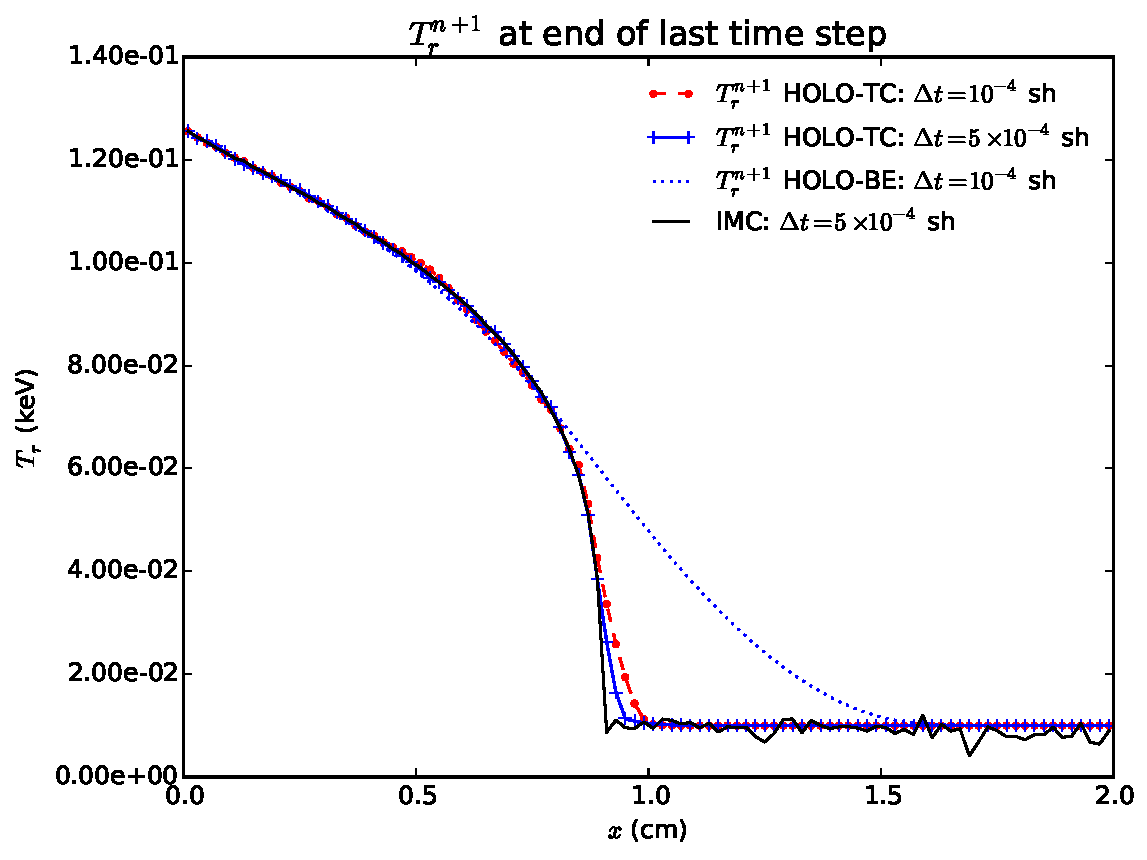
\includegraphics[width=0.75\textwidth]{thin_temp_compare.pdf}
    \caption{\label{fig:thin_temp_compare} Comparison of radiation temperatures of IMC and
    the HOLO method for different time step sizes and numbers of batches, for optically
thin problem. }
\end{figure}

Table.~\ref{tab:fom_thin} compares computed FOM values for the census
radiation energy densities, for the case of $\Delta t =
0.0005$~sh.  HOLO results were generated for the case of 1 and 2 batches, with the same
total number of histories per time step.  At low particle counts for the larger time step
size, the HOLO-TC method
demonstrates substantial noise.  This is due to the trial space representation of the
census particles at the end of the time step being poorly estimated.  For the 2 batch
case, the estimate from the first batch leads to less error in the census estimate as the
ECMC solves are simply solving for the deviation from the time-averaged quantity.  The
results for the case of 30,000 histories are plotted in Fig.~\ref{} for the HO and LO
solution.  As demonstrated, there seems to have been some instabilities introduced into
the LO equations through noise; sufficient sampling of the census must occur.
At smaller time-steps there is an increase in statistical efficiency, however there has
been a loss in accuracy due to an increase in projection error.  In general, this is a
balance that much be considered.

The accuracy of the HOLO-ECMC method was compared to a reference solution from IMC. This
problem is thin enough that we expect IMC to be accuracy with sufficient particle
histories.  The
reference solution is the average of 20 IMC simulations of $20\times10^6$
histories, each with $\delta t =10^{-4}$ sh.  The estimated value of $\ss$ for the
reference solution is 0.025\%.  The L$_2$ norm of the error in cell-averaged mean
intensities is computed 
at the end of the last time step, was computed.  The average over 20 simulations is then
computed to provide the metric
\begin{equation}
    \|e\|^l = \left({\frac{\sum\limits_{i=1}^{N_c}
    \left(\phi_i^{n+1,l} - \phi_i^{n+1,ref}
\right)^2}{\sum\limits_{i=1}^{N_c}\left(\phi_i^{n+1,ref}\right)^2}}\right)^{1/2},
\end{equation}
where $\phi_i^{n+1,l}$ is the cell-averaged scalar intensity at the end of the last time
step from the $l$-th independent simulation.  The sample mean of $\|e\|$ from 20
independent simulations provides a metric for the accuracy of a particular simulation:
\begin{equation}
    \overline{\|e\|} = \frac{1}{20}\sum_{l=1}^{20} \|e\|^l
\end{equation}

The accuracy results for 

\begin{table}[H]
\centering
\caption{\label{tab:fom_thin} {Comparison of sample statistics for the
    end of time step radiation energy densities, of the last time step, for the optically
    thin problem and $\Delta t = 5\times 10^{-4}$ sh.   Simulation end time is $\mathbf{t=0.003}$ sh.}}
\vspace{-0.1in}
\begin{tabular}{|c|ccc|ccc|}\cline{2-7}
    \multicolumn{1}{c|}{}       & \multicolumn{3}{|c|}{\ss} &
    \multicolumn{3}{|c|}{\FOM} \\ \hline
hists./step   & IMC & HOLO-TC (1) & HOLO-TC (3) &  IMC   & HOLO-TC(1) & HOLO-TC(3) \\ \hline
   30,000     & 3.01\%  & 18.29\% & 5.38\%      &  1.00  & 0.03  &  0.31      \\
  300,000     & 0.99\%  & 0.81\%  & 0.74\%      &  0.93  & 1.38  &  1.65     \\ 
  1,000,000   & 0.50\%  & 0.30\%  & 0.37\%      &  1.10  & 3.42  &  2.0      \\ \hline
\end{tabular}
\end{table}

\begin{table}[H]
\centering
\caption{\label{tab:thin_short} {Comparison of sample statistics for the
    end of time step radiation energy densities, of the last time step, for the optically
    thin problem and $\Delta t = 1\times 10^{-4}$ sh.   Simulation end time is $\mathbf{t=0.003}$ sh.}}
\vspace{-0.1in}
\begin{tabular}{|c|ccc|ccc|}\cline{2-7}
    \multicolumn{1}{c|}{}       & \multicolumn{3}{|c|}{\ss} &
    \multicolumn{3}{|c|}{\FOM} \\ \hline
hists./step   & IMC & HOLO-TC (1) & HOLO-TC (3) &  IMC   & HOLO-TC(1) & HOLO-TC(3) \\ \hline
   30,000     & 3.00\%  & 0.55\% & 1.28\%       &  1.00  &  29.81    & 5.51    \\
  300,000     & 0.96\%  & 0.11\% & 0.30\%       &  0.98  &  71.82    & 9.88    \\ 
  1,000,000   & 0.49\%  & 0.06\% & 0.17\%       &  1.11  &  71.02    & 9.71    \\ \hline
\end{tabular}
\end{table}


\section{Marshak Wave Problem}

It is important to demonstrate that the time closures are stable in a mix of optically
thick and optically thin regions, and that the ECMC method is still efficient in such
problems.  Simulations were performed for the Marshak wave problem defined in
Sec.~\ref{sec:marshak}.  The time step size is linearly increased from $0.001$ sh to a
maximum step of 0.01 sh over the first 10 time steps; the last time step is adjusted to
reach the desired simulation end time.  It was found for this problem that it was
necessary to use more than one batch for the HOLO-TC algorithm to stably converge.
This is because in the case of a single batch particles must reach
census to accurately estimate the next time step value.  These results were generated using the implicit-like time
closure.

\begin{figure}[H]
    \centering
    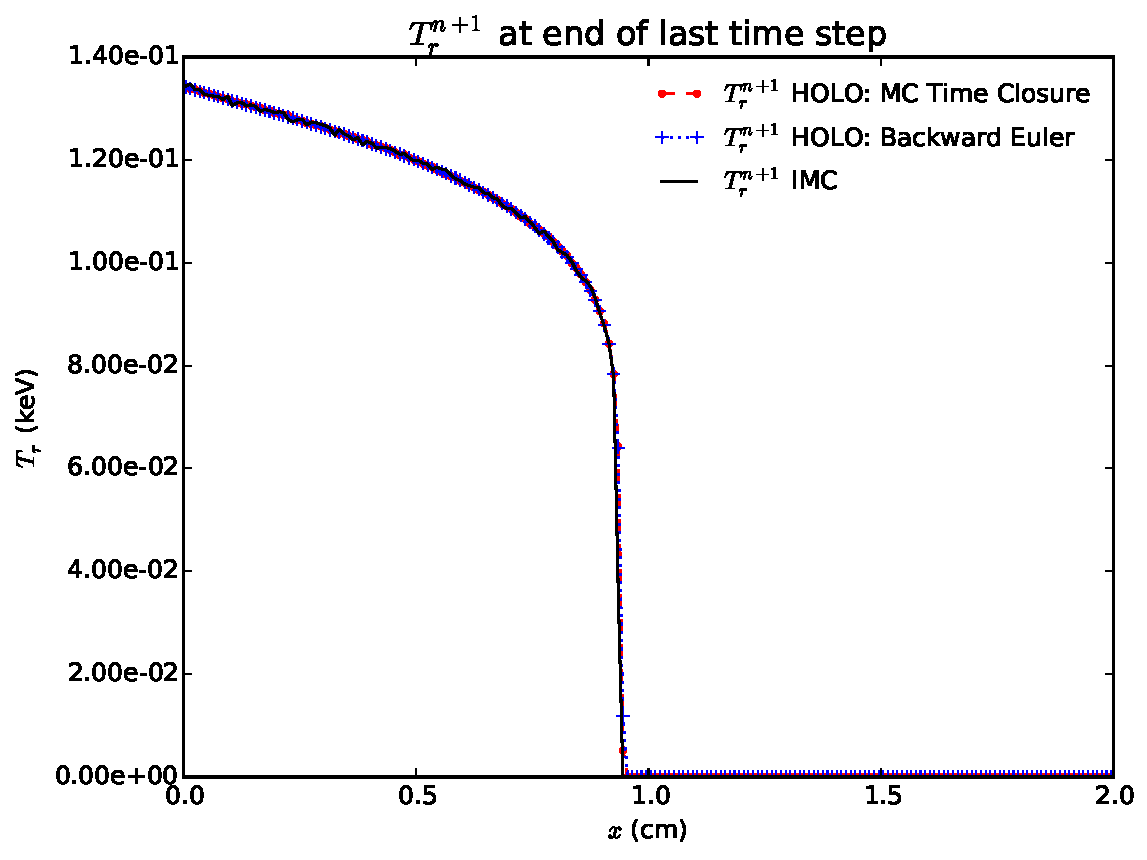
\includegraphics[width=0.65\textwidth]{marshak_time_cont_compare.pdf}
    \caption{\label{fig:marshak_tc} Comparison of HOLO-TC, HOLO-BE, and IMC methods for
the Marshak Wave problem, with $10^6$ histories per time step.}
\end{figure}

Figure~\ref{fig:marshak_tc} compares the accuracy of IMC, HOLO-TC, and HOLO-BE.  The
solutions are plotted at $t=3$ sh, with $10^6$ histories per time step for all
simulations. As demonstrated, there is good agreement among the results.  It is noted that
this problem can be accurately modeled with the Backward Euler time discretization, but
the MC time closure appears to be stable even in the mix of optically thick and thin
regions. Table~\ref{tab:marshak_cont} compares sample statistics for IMC and
the HOLO method with continuous time treatment and with a BE discretization.  As
demonstrated, at the lower history count (300,000), the HOLO-TC algorithm demostrates a
greater variance.  These results used the implicit
like time closure.

\begin{table}[H]
\centering
\caption{\label{tab:marshak_cont} {Comparison of sample statistics for the
    end of time step radiation energy densities, of the last time step, for the marshak
    wave problem and maximum time step of $0.01$ sh.  Simulation end time is $\mathbf{t=3.0}$ sh.}}
\vspace{-0.1in}
\begin{tabular}{|c|ccc|ccc|}\cline{2-7}
    \multicolumn{1}{c|}{}       & \multicolumn{3}{|c|}{\ss} &
    \multicolumn{3}{|c|}{\FOM} \\ \hline
hists./step   & IMC & HOLO-TC (2) & HOLO-BE (2) &  IMC   & HOLO-TC (2) & HOLO-BE (2) \\ \hline
  300,000     & 2.25\%  & 3.42\% & 0.30\%       &  1.00  &   0.43    & 2050          \\  
  1,000,000   & 1.27\%  & 0.31\% & 0.17\%       &  0.94  &  15.95    & 1806          \\ \hline
  \multicolumn{7}{|c|}{Diamond Like Closure} \\ \hline
  300,000     & --  & 3.53\% & --   &  --  &   0.41   & --  \\  
  1,000,000   & --  & 0.37\% & --   &  --  &  10.94   & --  \\ \hline
\end{tabular}
\end{table}


The importance sampling algorithm
detailed in Sec.~\ref{sec:imp_sampling} was investigated for this problem set up.  In
particular, various values of $p_{surv}$ with a fixed value of 2 mfp of survival distance
were investigated.  Sample statistics were measured for the HOLO-TC algorithm and the case of two batches of
100,000 histories per time step, with a max time step of 0.01 sh.    The importance
sampling algorithm was found to generally increase the variance, for this problem.  This
is likely caused by the fact that when no importance sampling is used, in the very thick
cells essentially no particles reach the census.  In such cells, because the ECMC
algorithm is estimating the difference between the first batch's estimate of
$\overline{I}(x,\mu)$ and $\tilde I^{n+1}(x,\mu)$, it just accepts $\overline I(x,\mu)$ as
$I^{n+1}(x,\mu)$.  The initialization of the solution to the first batches estimate of
$\overline{I}(x,\mu)$ is sufficient to produce visually accurate results because the waves
are moving so slowly. When importance sampling is used, 
There is likely a regime of problems where it is necessary to
sample the census more thoroughly and the importance sampling may reduce variance.  



\begin{table}[H]
\centering
\caption{\label{tab:void_short} {Comparison of sample statistics using importance
    sampling on the interior of the time step, for the Marshak Wave problem.  Simulation
    end time is $\mathbf{t=1.0}$ sh.} and max $\Delta t$ is 0.01 sh}
\vspace{-0.1in}
\begin{tabular}{|cc|} \hline
        $p_{surv}$ & {\FOM} \\ \hline
       No Bias & 1 \\ 
       0.05    & 0.001 \\
       0.1     & 0.005 \\
       0.25    & 0.179  \\
       0.5     & 0.003 \\ \hline
\end{tabular}
\end{table}









